\chapter{Mutant npat results in nucleosome positioning defects in \textit{D. rerio} CMZ progenitors, blocking fate specification but not proliferation}
\chaptermark{Nucleosome position and specification defects in npat mutant \textit{rys}}
\label{chap:rys}
\section{Introduction}
The zebrafish (\textit{D. rerio}) circumferential marginal zone (CMZ), located in the retinal periphery, contains the retinal stem cells and progenitors responsible for the lifelong retinal neurogenesis observed in this cyprinid. Analagous to CMZs in other model organisms, such as \textit{X. laevis} \cite{Perron1998}, it has been of particular interest to us since the discovery of quiescent stem cells at the mammalian retinal periphery \cite{Tropepe2000}, as an understanding of the molecular regulation of this proliferative zone may shed light on whether these mammalian cells might be harnessed for the purpose of regenerative retinal medicine. While significant progress has been made in this direction \cite{Raymond2006}, molecular lesions in a plethora of zebrafish mutants displaying defects in CMZ development and activity remain largely uncharacterised. We examine here one such micropthalmic line identified in an ENU screen, \textit{rys} \cite{Wehman2005}, characterised by Wehman et al. as a Class IIA CMZ mutant, with a small eyes (see \autoref{ryspic}) and apparently paradoxically enlarged CMZ.

\begin{figure}[!h]
    \makebox[\textwidth][c]{\includegraphics[width=.6\textwidth]{rys/rys.jpg}}    
    \caption{{\bf \textit{rys} mutants exhibit a small-eye phenotype}}
    \label{ryspic}
    8 dpf \textit{rys} sibling (Sib) and mutant (Rys), head area (top panels), whole body (bottom panels). Red dashes highlight the overall reduced eye size in homozygous \textit{rys} mutant animals.
\end{figure}

Mapping revealed the causative \textit{rys} mutation in the zebrafish npat gene, the nuclear protein associated with the ataxia-telangiectasia locus in mammals \cite{Imai1996}. Although npat is heretofore uncharacterised in zebrafish, its mammalian homologues, human NPAT and mouse Npat, have been extensively examined. These studies demonstrated that NPAT plays a critical role in coordinating events associated with the G1/S phase transition in proliferating cells \cite{Ye2003}. S-phase entry requires tight co-ordination between the onset of genomic DNA synthesis and histone production, in order to achieve normal chromatin packaging and assembly. NPAT, found in the nucleus \cite{Sagara2002} and localised, in a cell-cycle dependent manner, to histone locus bodies \cite{Ghule2009}, induces S-phase entry \cite{Zhao1998} and activates replication-dependent histone gene transcription by direct interaction with histone gene clusters \cite{Zhao2000} in association with histone nuclear factor P (HiNF-P) \cite{Mitra2003}. The protein’s effects on S-phase entry and histone transcription are associated with distinct domains at the C-terminus and N-terminus, respectively \cite{Wei2003}. NPAT is also known to associate with the histone acetyltransferase CBP/p300 \cite{Wang2004} and directs histone acetylation by this enzyme \cite{He2011}.

NPAT is involved in E2F transcriptional regulation \cite{Gao2003} and a is substrate of cyclin E/CDK2 \cite{Zhao1998}, although E2F-independent activation by cyclin D2/CDK4 in human ES cells has also been described \cite{Becker2010}. The expression of NPAT protein peaks at the G1/S boundary \cite{Zhao1998}, as does its phosphorylation, which promotes its transcriptional activation of replication-dependent H2B \cite{Ma2000} and H4 \cite{Mitra2009} genes, while its effect on low, basal levels of H4 transcription is phosphorylation-independent \cite{Ye2003}. Of particular interest, NPAT has recently been found to be required for CDK9 recruitment to replication-dependent histone genes \cite{Pirngruber2010}; CDK9 and monoubiquitinated H2B are essential for proper 3’ end processing of stem-loop histone transcripts \cite{Pirngruber2009}. NPAT and HiNF-P have also been found associated with the U7 snRNP complexes that perform this function \cite{Ghule2009}. The replication-dependent activities of NPAT are thought to be terminated by WEE1 phosphorylation of H2B, which excludes NPAT from histone clusters \cite{Mahajan2012}.

All of these studies were performed in tissue culture, perhaps due to the challenges associated with studying this critical protein in vivo; mouse embryos with provirally inactivated Npat arrest at the 8-cell stage, for instance \cite{DiFruscio1997}. The availability of \textit{rys}, a zebrafish npat mutant which develops well into the larval stage, is therefore of considerable interest, as it allows for the study of npat’s function within complete tissues. We demonstrate here that npat is critical for fate specification of CMZ neural progenitors. We find substantial evidence for the role of \textit{D. rerio} npat involvement with histone transcription, nucleosome positioning, and scheduling of mitotic activity; we suggest that the \textit{rys} phenotype is brought about by a failure to coordinate the genomic states required to specify, independently of proliferative capacity, in postembryonic zebrafish RPCs of the CMZ.

\section{Results}
\subsection{The \textit{rys} CMZ phenotype is characterised failure of RPCs to specify, altered nuclear morphology, aberrant proliferation and expanded early progenitor identity}

\textit{rys} has an enlarged CMZ \cite{Wehman2005}, but whether this is a consequence of more RPCs, larger RPCs, or other causes, is unknown. We examined niche ontogeny during the early life of \textit{rys} animals using two histochemical markers of cycle activity: Proliferating Cell Nuclear Antigen (PCNA), which in \textit{D. rerio} is expressed throughout the cell cycle; and the genomic incorporation of the thymidine analogue EdU over a 24 hour pulse, marking passage through S-phase during this time. These data are displayed in \autoref{rysCMZontogeny}. During this period, the PCNA positive population of the sibling CMZ declines (Panel A), with a corresponding decrease in proliferative activity as measured by the incorporation of EdU (Panel B). Whether or not the mutant \textit{rys} CMZ population is enlarged by comparison depends on the age at which it is sampled. There is a 99.6\% probability that the posterior mean RPC population in mutants is less than the sib mean at 4dpf, while there is a 99.8\% probability of the 10dpf \textit{rys} mean being greater than that of sibs. Therefore, the \textit{rys} CMZ population is better described as achieving its peak periembryonic size later than siblings; its population is only numerically larger than sibs at later ages\footnote{\textit{rys} animals universally die by approximately 3 weeks of age.}. 

\begin{figure}[!h]
    \makebox[\textwidth][c]{\includegraphics[width=1.\textwidth]{rys/CMZontogeny.png}}    
    \caption{{\bf \textit{rys} CMZ populations start relatively small and quiescent, end abberantly large and proliferative}}
    Panel A: Counts and estimated mean $\pm$95\% credible intervals of PCNA-positive cells in the peripheral CMZ of \textit{rys} (magenta) and their siblings (green). Counts obtained from one 14 \si{\micro\metre} central coronal cryosection per individual.
    Panel B: As above, but for counts of double PCNA-,EdU-positive cells in the CMZ after a 24 hour pulse of EdU.
    \label{rysCMZontogeny}
    Methods in \autoref{ssec:rysPCNAEdU}.
    Code in \autoref{ssec:ryspont}.
\end{figure}
\FloatBarrier

Few \textit{rys} RPCs are actively cycling at 4dpf, by comparison to the rapidly proliferating sibling cells; a mean estimate of 96.2$\pm$3.4\% of sib RPCs are labelled during the 24 hr pulse at 4dpf, while only 24.1$\pm$37.2\% of \textit{rys} RPCs are. The situation is broadly reversed at 10dpf, with only 24.4$\pm$14.9\% of sib RPCs labelled, compared to 65.8$\pm$16.2\% of \textit{rys} RPCs. Confirming this late-stage increase in \textit{rys} thymidine analogue labelling represents bona fide mitotic activity, we found mitotic figures in labelled mutant RPCs at 10dpf, shown in Supplementary \autoref{rysmitosis}. In \textit{rys} animals which have actively proliferating RPCs at early ages, the CMZ fails to contribute to the central neural retina. Confocal micrographs displaying \textit{rys} CMZ cohorts labelled with BrdU at 3dpf that have failed to enter the neural retina after 7 days of chase time are displayed in \autoref{contributionfailure}. 

\begin{figure}[!h]
    \makebox[\textwidth][c]{\includegraphics[width=1.\textwidth]{rys/cmzfailure.png}}    
    \caption{{\bf \textit{rys} CMZ RPCs fail to contribute to the neural retina}}
    14\si{\micro\metre} coronal cryosections through representative sib (left panels) and \textit{rys} (right panels) eyes at 10dpf, 7 days after an 8hr BrdU pulse at 3dpf. Green: anti-BrdU labelling. Blue: Hoechst 33342 counterstain.
    Methods in \autoref{ssec:rysBrdUpulse}.
    \label{contributionfailure}
\end{figure}
\FloatBarrier

The thymidine analogue pulse-chase studies described above give little direct information about cell cycle characteristics, so we performed a cumulative thymidine labelling experiment in \textit{rys} mutants and siblings at 5dpf, when similar proportions of the PCNA+ve CMZ population retain thymidine label. We inferred cycle parameters by nested sampling, using the thymidine slice model simulator presented in \autoref{chap:CMZ}. Kernel density estimates of relevant cycle posterior distributions are presented in \autoref{a35kdes}, while maximum a posteriori model output for sib and mutant data are presented in Supplementary \autoref{a35sibMAP} and \autoref{a35rysMAP}, respectively. 

\begin{figure}[!h]
    \makebox[\textwidth][c]{\includegraphics[width=.7\textwidth]{rys/a35marginals.png}}    
    \caption{{\bf \textit{rys} CMZ RPCs fail to contribute to the neural retina}}
    14\si{\micro\metre} coronal cryosections through representative sib (left panels) and \textit{rys} (right panels) eyes at 10dpf, 7 days after an 8hr BrdU pulse at 3dpf. Green: anti-BrdU labelling. Blue: Hoechst 33342 counterstain.
    Methods in \autoref{ssec:rysBrdUpulse}.
    \label{a35kdes}
\end{figure}

Examining 5dpf CMZ RPC nuclear number and morphology (\autoref{nuclearstudy}) suggests the enlarged appearance of \textit{rys} CMZs is the failure to contribute to the neural retina, leading to \textit{rys} RPCs contributing half as many central neurons as their siblings (Panel B), despite having similar overall populations at his age (Panel A). This appearance may be enhanced in the dorsal CMZ population, which tends to be more numerous in \textit{rys} than sibs, although this tendency is reversed in the ventral population (Panels C and D). More significantly, \textit{rys} nuclei are usually larger than their siblings (Panel E), as well as consistently less spherical (Panel F).

\begin{figure}[!h]
    \makebox[\textwidth][c]{\includegraphics[width=1.\textwidth]{rys/nuclearstudy.png}}    
    \caption{{\bf 7dpf \textit{rys} CMZ RPCs display enhanced asymmetry, increased volume, decreased sphericity, and relative but not absolute enlargement}}
    \label{nuclearstudy}
    All panels display sib observations as green circles and \textit{rys} as magenta triangles. Plotted behind the underlying observations are the calculated marginal posterior distributions of the mean, given log-Normal models of the population data and Normal models of the volume and sphericity data. The y-axis shows the relative likelihood of underlying mean values on the x-axis, given the data.
    Panel A: Total PCNA-positive RPC population per central coronal section.
    Panel B: Number of PCNA negative, specified central retinal neurons per PCNA postive RPC.
    Panels C and D: Dorsal and Ventral RPC populations per central coronal cryosection.
    Panel E: Mean volume of nuclei in a given individual's central coronal cryosection.
    Panel F: Mean sphericity of nuclei in a given individual's central coronal cryosection.
    Methods in \autoref{ssec:rysPCNAEdU}.
    Code in \autoref{ssec:a38}.
\end{figure}

To rank these contributions to the \textit{rys} nuclear phenotype, we calculated the \hyperref[ssec:BayesEpistemology]{Bayesian evidence} (marginal probability) for combined Log-Normal (population measurements) and Normal (nuclear measurements) models of sib and rys data, against the joint evidence for separate models. These estimates are presented in \autoref{nuclearev}. Of the effects that differentiate \textit{rys}from sibs (positive evidence ratio, logZR in \autoref{nuclearev}), the largest is decreased nuclear sphericity, followed by decreased nuclear volume. These are followed by differences in dorsal and ventral CMZ populations, then by the mutant's decreased number of central retinal neurons relative to the RPC population. These models suggest the nuclear morphological changes are the most important contributors to the \textit{rys} enlarged-CMZ phenotype.

\begin{table}[!ht]
    \centering
    \caption{{\bf Evidence-based ranking of phenomenal contributors to \textit{rys} phenotype}}
    \begin{tabular}{|l|l|l|l|l|} 
        \hline {\bf Parameter} & {\bf Separate rys-sib logZ} & {\bf Combined rys-sib logZ} & {\bf logZR} & {\bf $\sigma$ sign.}\\ \hline 
        Sectional CMZ pop. & -299.9 ± 1.1 & {\bf -203.4 ± 1.0} & -96.6 ± 1.5 & -65.4 \\ \hline
        Central pop./RPC  & {\bf -56.11 ± 0.27} & -79.52 ± 0.17 & 23.41 ± 0.32 & 73.7 \\ \hline 
        Dorsal CMZ pop. & {\bf -175.7 ± 0.92} & -228.4 ± 1.4 & 52.7 ± 1.6 & 32.2 \\ \hline 
        Ventral CMZ pop. & {\bf -136.6 ± 0.24} & -167.15 ± 0.13 & 30.55 ± 0.27 & 113.8 \\ \hline 
        Nuclear Volume & {\bf -164.57 ± 0.22} & -224.3 ± 1.7 & 59.7 ± 1.7 & 34.4 \\ \hline 
        Nuclear Sphericity & {\bf -87.19 ± 0.27} & -265.5 ± 2.3 & 178.3 ± 2.3 & 78.4 \\ \hline
    \end{tabular}
    \begin{flushleft}
    logZ: logarithm of p(D), the marginal likelihood of the data, or model evidence. logZR: evidence ratio; positive ratios in favour of separate modelling of the sib and \textit{rys} 
    data. Largest evidence values bolded.
    Methods in \autoref{ssec:rysnucev}.
    Code in \autoref{ssec:rysp_GMC_NS}.
    \end{flushleft}
    \label{nuclearev}
\end{table}

\FloatBarrier

\begin{figure}[!h]
    \makebox[\textwidth][c]{\includegraphics[width=.8\textwidth]{rys/rysem.png}}    
    \caption{{\bf RPC nuclei of the \textit{rys} CMZ display disorganized, loosely packed chromatin}}
    Representative electron micrographs of \textit{rys} sibling and mutant CMZ RPC nuclei.
    Left panels: siblings. Right panels: \textit{rys}. Top panels: 36000x magnification, general overview of the area around the nucleus, dashed black. Area displayed in middle panels dashed white. Middle panels: 110000x magnification nuclear detail. Area displayed in bottom panels dashed white. Bottom panels: 210000x magnification, chromosomal ultrastructure.
    Methods in \autoref{ssec:rysEM}.
    \label{rysEM}
\end{figure}

Enlarged \textit{rys} RPC nuclei have a billowy appearance suggestive of chromosomal disorganization. We used electron microscopy to examine the nuclear ultrastructure of RPC nuclei in \textit{rys} and sibling CMZs. Representative electron micrographs are presented in \autoref{rysEM}. At 36000x magnification, the stretched and pancaked structure of \textit{rys} nuclei is apparent, in contrast with the consistently teardrop-shaped nuclei of sibling RPCs. When the chromatin is imaged at 210000x magnification, it appears less electron-dense in \textit{rys} mutants, with larger tracts of presumptive euchromatin, and less regular spacing of chromosomal material.
\FloatBarrier

If RPCs in \textit{rys} CMZs fail to enter the specified neural retina, but by 7dpf are becoming mitotically active, an explanation for the proliferative niche's population declining by 10dpf is required. We suspected \textit{rys} RPCs may be apoptosing in situ. Although we did not detect pyknotic nuclear fragments in our EM investigations, it may be that the apoptotic events are too rare in \textit{rys} to detect in this manner. We therefore assayed the presence of the apoptotic marker caspase-3 in \textit{rys} and sib CMZs. As displayed in \autoref{caspase}, caspase-3-positive nuclei can be detected in the \textit{rys} CMZ at both 4 and 6 dpf (mean 6.5 $\pm$ 7.5 and 2.6 $\pm$ 1.1 cells, respectively) but are not found in sib CMZs, though both display a similar level of central apoptotic activity (4dpf \textit{rys}: 1.25 $\pm$ 1.0; 4dpf sib: 1.4 $\pm$ 1.1; 6dpf \textit{rys} 0.6 $\pm$ 0.9; 6dpf sib: 1.0 $\pm$ 1.4 ). The lack of debris observable in \textit{rys} CMZs is likely attributable to the activity of 4C4-positive microglia active in the area; we observed one such cell actively phagocytosing TUNEL-labelled \textit{rys} RPC nuclear fragments in the CMZ, displayed in Supplementary \autoref{phagocytosis}.

\begin{figure}[!h]
    \makebox[\textwidth][c]{\includegraphics[width=1.\textwidth]{rys/caspase.png}}    
    \caption{{\bf \textit{rys} mutant CMZs have increased caspase-3 positive nuclei}}
    Number of caspase-3 positive nuclei counted in CMZ, the border between the CMZ and specified central retina, the specified central neural retina, and the overall total, at 4 dpf (left panel) and 6 dpf (right panel). One central \SI{20}{\micro\metre} section per sibling (S) and \textit{rys} (R) larva.
    \label{caspase}
    Methods in \autoref{ssec:ryscaspase}.
    Code in \autoref{ssec:caspasescript}.
\end{figure}

Suspecting that \textit{rys} CMZ RPCs may maintain an early progenitor identity, we examined pax6a immunostaining of this population, which is normally restricted to putative progenitors in the peripheral and middle CMZ, as well as the retinal ganglion cell layer \cite{Raymond2006}. The Pax6-stained region was enlarged in \textit{rys} CMZs relative to their siblings (\autoref{progenitoridentity}, center panels). As vsx2 is also known to be a marker of retinal progenitor cells in the CMZ \cite{Raymond2006}, we also generated a transgenic vsx2::eGFP \textit{rys} line, which produces eGFP expression in the utmost retinal periphery in siblings. Mutant fish from this line displayed substantially expanded eGFP expression in the CMZ (\autoref{progenitoridentity}, right panels).

\begin{figure}[!h]
    \makebox[\textwidth][c]{\includegraphics[width=1.2\textwidth]{rys/progenitorid.png}}    
    \caption{{\bf Mutant \textit{rys} RPCs display expanded expression of early progenitor markers}}
    Representative transmitted light and confocal micrographs of \textit{rys} sibling and mutant CMZ RPCs. Top panels: siblings. Bottom panels: \textit{rys} mutants. Left panels: in-situ hybridization using npat probe (blue) on 20\si{\micro\metre} coronal cryosections. Middle panels: anti-Pax6 (red) on Hoechst 33342 nuclear counterstain. Right panels: anti-GFP (green) on Hoechst 3342 nuclear counterstain, in a Tg(vsx2:GFP) line introgressed into \textit{rys}. 
    Methods in \autoref{ssec:rysprogenIHC}, \autoref{ssec:rysISH}.
    \label{progenitoridentity}
\end{figure}

\FloatBarrier
\subsection{The micropthalmic zebrafish line \textit{rys} is an npat mutant}

We performed linkage mapping to identify the causative mutation responsible for the \textit{rys} phenotype, followed by PCR analysis of the transcript products of candidate genes. This study revealed a single G\textgreater{}A transition at position 24862961 on chromosome 15 (NC\_007126.5, Zv9), annotated as the first base of intron 9 in the zebrafish npat gene, in a canonical GU splice donor site. 

We observed that this mutation reliably results in the retention of npat intron 8, and, less frequently, in the retention of both introns 8 and 11, in 6dpf \textit{rys} mutants, shown in \autoref{npattranscript}. The predicted mutant protein is truncated by a stop codon at residue 283, which would preclude the translation of predicted phosphorylation sites and nuclear localisation signals cognate to those identified in human NPAT \cite{Ma2000,Sagara2002}, as displayed in \autoref{npatprotein}.

\begin{figure}[!h]
    \makebox[\textwidth][c]{\includegraphics[width=.8\textwidth]{rys/PCRE8-E11WtSibRys.jpg}}    
    \caption{{\bf RT-PCR analysis reveals two aberrant intron retention variants in \textit{rys} mutant npat transcripts}}
    \label{npattranscript}
    Top panel: Agarose gel electrophoresis of mRNAs prepared from 3dpf homozygous wild type (+/+), heterozygote (+/-), and homozygous mutant (-/-) animals, as identified by genomic PCR. Fragments were amplified from a forward primer sited in exon 8 and a reverse primer sited in exon 11.
    Bottom panel: exon/intron layout schematics of the putative transcripts detected.
    Methods in \autoref{ssec:rysPCR}.
\end{figure}

\begin{figure}[!h]
    \makebox[\textwidth][c]{\includegraphics[width=.8\textwidth]{rys/Npat protein.jpg}}    
    \caption{{\bf Functional domains of Human NPAT compared to predicted wild-type and \textit{rys Danio} npat}}
    Proteins presented as linear domain schematics with number of amino acids along the horizontal axis.
    \label{npatprotein}
\end{figure}
\FloatBarrier

Because \textit{D. rerio} is a teleost known to have undergone genome duplication in an ancestral clade, we used the Synteny Database tool \cite{Catchen2009} identify any possible npat duplicates. A duplicated gene could explain the lessened severity of the mutant \textit{Danio} phenotype when compared to mammalian proviral inactivants. The results of this analysis are presented in Supplementary \autoref{synteny}. While npat is in the midst of a region which appears to be duplicated on chromosomes 5 and 15, relative to the homologous syntenic run on \textit{H. sapiens} chromosome 11, it is not, itself, duplicated.

We performed in situ hybridisation against npat transcript to confirm that the gene is indeed expressed in wild type CMZs; we found that npat expression is progressively restricted to the CMZ from 4 to 6 dpf in wild-type fish. A representative time-course of 20 \si{\micro\metre} cryosections through ISH-treated embryos is depicted in \autoref{npatISH}, focusing on the retina at the times when it has formed. Although npat remains transcribed in both the specified GCL and amacrine-rich inner INL to a degree, it is most intensely expressed in the proliferative CMZ, as suggested by its cell cycle functions.

\begin{figure}[!h]
    \makebox[\textwidth][c]{\includegraphics[width=.8\textwidth]{rys/ISH.png}}    
    \caption{{\bf In situ hybridization reveals progressive restriction of npat expression to the CMZ}}
    20\si{\micro\metre} sections of wild-type embryo (1dpf) and retinae (4 and 6 dpf), displaying progressive restriction of npat expression (blue) as assayed by in-situ hybridisation.
    Methods in \autoref{ssec:rysISH}.
    \label{npatISH}
\end{figure}

Given unusual chromatin ultrastructure in \textit{rys} CMZ RPCs, and npat's role in histone regulation, we investigated the transcriptional status of npat and its histone regulatory targets by RT-PCR. Homozygous \textit{rys} mutants overtranscribe npat by about 3-fold compared to their wild-type counterparts at both 6dpf and 8dpf. Sibling overabundance compared to wild-type declines from about 2.5-fold to 1.5-fold over this time period, as shown in Supplementary \autoref{npatrtpcr}.

Since mammalian NPAT regulates histone transcription and is critical for coordinating expression of replication-dependent histones required to package genomic DNA during S-phase \cite{Zhao2000}, we hypothesized that the altered nuclear morphology we observed in \textit{rys} CMZ RPCs may be a consequence of perturbed histone transcription. To test this, we performed qPCR on random-hexamer-primed cDNAs produced from 6 and 8dpf wild type, sibling, and \textit{rys} embryo mRNA extracts. These qPCR assays were performed using degenerate primers\footnote{Zebrafish have notably populous histone clusters with numerous variants and pseudogenes not present in non-genomically-duplicated vertebrates, so degenerate primers are an appropriate way to survey the population of transcripts. A full catalogue has not been undertaken, to my knowledge.} directed toward zebrafish core histone gene families H2A, H2B, H3 and H4. As a role for NPAT in 3’ end processing of histone transcripts has been identified \cite{Pirngruber2010}, we also set out to determine whether 3’ end processing of histone transcripts is altered in \textit{rys}. By repeating these qPCR assays on oligo-dT-primed cDNAs, we examined the population of polyadenylated histone transcripts in isolation. 

\begin{figure}[!h]
    \makebox[\textwidth][c]{\includegraphics[width=.8\textwidth]{rys/qPCR.png}}    
    \caption{{\bf \textit{rys} overexpress total and polyadenylated core histone transcripts}}
    qPCR results for degenerately-primed families of core histone total transcripts (left panels), and polyadenylated transcripts (right panels). From top to bottom, H2A, H2B, H3, and H4 family results are displayed in separate panels. Animal age in dpf on the x axis, fold change vs. wild-type standard on the y axis.    
    \label{histonertpcr}
    Methods in \autoref{ssec:rysqPCR}.
    Code in \autoref{ssec:qPCR}.
\end{figure}

These results demonstrated that both mutant \textit{rys} and siblings overexpress histone transcripts to various degrees. In order to determine which histone families are most plausibly involved in the \textit{rys} mutant phenotype, we calculated the statistical significance for mean rys transcript levels exceeding mean sibling transcript level or the WT standard (set to 1.0). To be implicated in the phenotype, mutant transcript levels should be higher than both siblings and wild-type animals. We used a cutoff of 2 SDs of significance for both the sibling and WT tests for a given transcript family. These values are presented in \autoref{qPCRstds}.

\begin{table}[!ht]
    \centering
    \caption{{\bf Standard deviations of significance for \textit{rys} mutant transcript $>$ sib or WT}}
    \begin{tabular}{|l|l|l|l|l|l|} 
        \hline {\bf Transcript} & {\bf Age} & \multicolumn{2}{c|}{\bf{Total}} & \multicolumn{2}{c|}{\bf{polyA}}\\ \cline{3-6}
        {\bf Family} & {\bf (dpf)} & {\bf Sib mean $\sigma$} & {\bf WT std $\sigma$} & {\bf Sib mean $\sigma$} & {\bf WT std $\sigma$}\\ \hline 
        H2A & 6 & 1.59 & 3.72 & 1.68 & 1.68\\ \hline
        H2A & 8 & {\bf 2.75} & {\bf 5.4} & {\bf 2.18} & {\bf 2.3}\\ \hline
        H2B & 6 & {\bf 2.12} & {\bf 2.37} & 1.47 & 1.52\\ \hline
        H2B & 8 & 1.9 & 7.59 & {\bf 2.76} & {\bf 2.89}\\ \hline
        H3 & 6 & 0.77 & 3.39 & 0.6 & 0.97\\ \hline
        H3 & 8 & 1.21 & 1.83 & 0.78 & 0.54\\ \hline
        H4 & 6 & -0.26 & -0.58 & 1.15 & 1.46\\ \hline
        H4 & 8 & 0.79 & 8.83 & 0.45 & 0.35\\ \hline
    \end{tabular}
    \caption{    \label{qPCRstds}
    Standard deviations of significance for differences between mean \textit{rys} mutant transcript expression, relative to siblings or WT standard (1.0), at 6 and 8 dpf. Values for histone transcript pools with \textgreater2 SDs of significance for both sib and WT tests in bold. 
    Methods in \autoref{ssec:rysqPCR}.
    Code in \autoref{ssec:qPCR}.
    }
\end{table}

Both total and polyadenylated \textit{rys} H2A are overexpressed in mutants relative to both siblings and WT controls at 8 dpf, while total H2B is overexpressed at 6dpf and polyadenylated H2B at 8dpf, using the criterion of 2 SDs of significance on both tests. We note that the overabundances of polyadenylated H2A and H2B are approximately 2-20 fold greater than those observed for any other transcript pool or histone family. 

The joint probability that mean \textit{rys} mutant total H2A is greater than the sib mean at both 6dpf and 8dpf to be 99.7\% $\pm$ 5.0; the same figure for H2B is 98.5\% $\pm$ 5.1. The joint probability that mean total H2A and H2B are elevated in \textit{rys} mutants compared to sibs at both ages is therefore 98.2\% $\pm$ 7.1. For the polyadenylated transcripts, the joint probability that the \textit{rys} mutant polyA H2A mean is greater than the sib mean at both ages is 94.1\% $\pm$ 9.9; the same figure for H2B is 92.6\% $\pm$ 3.3. The joint probability that mean polyadenylated H2A and H2B are elevated in \textit{rys} relative to sibs at both ages is then 87.1\% $\pm$ 9.7. 

On the basis of these calculations, the most plausible causal contributors to the \textit{rys} phenotype are H2A and H2B family transcripts. While the relative magnitude of total H2A and H2B transcript overexpression is less than that of the polyadenylated pool, we have less uncertainty about these figures. Still, the polyadenylated transcript results suggest mutant npat increases polyadenylation of these transcripts, possibly as a result of a loss of regulation of this system. Unlike the total transcript pool, siblings retain tight, WT-like control over polyadenylated transcripts. \textit{rys} mutants display much more extensive variability in polyA transcript expression, even where the mean is not elevated above siblings or WT controls.

\begin{figure}[!h]
    \makebox[\textwidth][c]{\includegraphics[width=.7\textwidth]{rys/morpholinos.jpg}}    
    \caption{{\bf 48hpf embryos injected with an npat ATG-targeted morpholino display a small-eye phenotype}}
    48 hpf wild-type embryos injected at the 1-2 cell stage with a control morpholino (CTRL), a morpholino targeting the npat splice site affected by the \textit{rys} mutation (Spl MO), and a morpholino targeting the npat start codon (ATG Mo).
    Methods in \autoref{ssec:moinjxn}.
    \label{morpholinopics}
\end{figure}

We further investigated npat's involvement by perturbing its transcription using morpholino injections of wild-type (AB strain) fish. As we do not suppose early morpholino transcriptional blockade will exactly replicate the cellular conditions of a genetic null some days after birth, particularly given the maternal contribution of npat transcript \cite{Harvey2013}, we did not seek to recapitulate the \textit{rys} phenotype. Rather, we sought to determine if any of \textit{rys}'s constituent phenomena would appear after an early blockage of \textit{rys} transcription, further substantiating the general involvement of npat in \textit{rys}. We tested morpholinos directed both to the npat start codon and to the splice site affected in \textit{rys}, alongside control morpholinos and uninjected animals. We used both a morpholino directed to the transcript ATG start site, as well as to the affected splice site. 

The splice morpholino replicated the \textit{rys} overexpression of both total and polyadenylated core histone transcript, while the ATG morpholino more narrowly replicated the effect on polyadenylated transcript (\autoref{morpholinoRTPCR}). The ATG morpholino also produced some animals with small eyes by 72dpf, as shown in \autoref{morpholinopics}. We also conducted an analysis of the nuclear morphological parameters measured in \autoref{nuclearstudy} for \textit{rys} mutants and siblings. For each of the ATG and splice morpholinos, we estimated the joint evidence for separate experimental morpholino and control morpholino models against a combined model. The evidence calculations are presented in Supplementary \autoref{morpholinoev}. We found substantial evidence in favour of separate models for the ATG and control morpholino effects on the number of central retinal neurons per proliferating RPC, suggesting that the ATG morpholino tends to decrease CMZ contribution to the specified retina. This result is displayed in \autoref{morphonucstudy}; the effect is more subtle than that displayed by mutants in \autoref{nuclearstudy}. These results establish that the identification of npat as the causative mutation in \textit{rys} is plausible, as experimental perturbation to npat in WT fish can result in \textit{rys} phenotypic phenomena, notably overexpression of core histone transcripts and small eyes arising from a decrease in the population of the central retina without a concomittant decrease in CMZ population. 

\begin{figure}[!h]
    \makebox[\textwidth][c]{\includegraphics[width=.75\textwidth]{rys/morphnuclei.png}}    
    \caption{{\bf ATG morpholino perturbation of npat recapitulates decline in mean  central retinal population relative to CMZ}}
    Populations of 14\si{\micro\metre} central coronal cryosections from retinas of animals injected with control (green triangles), npat splice-directed (yellow diamonds), and npat start codon-directed (magenta circles), standardized by number of CMZ RPCs. Plotted behind the underlying observations are the calculated marginal posterior distributions of the mean, given log-Normal models of the data. The y-axis displays the relative likelihood of underlying mean values on the x-axis, given the data.
    Methods in \autoref{ssec:moinjxn}, \autoref{ssec:rysPCNAEdU}.
    Code in \autoref{ssec:a38GMC_NS}.
    \label{morphonucstudy}
\end{figure}

\subsection{\textit{rys} siblings and mutants have unique sets of nucleosome positions, best explained by different sequence preferences and increased sequence-dependent positioning in mutants}
 Perturbed histone expression in \textit{rys} embryos suggests disrupted chromatin organisation as an explanation for the mutant nuclear phenotype, a possible consequence of altering the dynamic composition of the histone pool available for nucleosome formation during cell cycle. We therefore characterised nucleosome positioning in \textit{rys} and wild-type siblings by micrococcal nuclease (MNase) digestion of pooled genomic DNA (gDNA) \cite{Cui2012}. Nucleosome-protected fragments from the MNase digests were sequenced and positions called as described previously \cite{Chen2013}.

 \begin{figure}[!h]
    \includegraphics{rys/proportional_chromosome_occupancy.png}
    \caption{{\bf \textit{rys} chromosomes are differentially enriched and depleted of nucleosome position density and occupancy.}}
    Pie charts of nucleosome position density and occupancy by chromosome. Width of pie slices in panels A and B indicates the fraction of the total number of positions occuring in the numbered chromosomes and nonchromosomal scaffolds (NC). In panel A, depicting the sib genome, slices are colored according to the extent of deviation from an assumption of even distribution of nucleosomes across the genome. In panel B, depicting the \textit{rys} genome, slices are colored according to the extent of deviation from the sib distribution. The width of slices in slices B and D indicate the fraction of the total nucleosome occupancy signal detected. Slice coloration depicts deviations from nucleosome occupancy distributions analogous to position distributions in A and B. Blue and white diagonal bars in the NC slice of panel C denote an out-of-scale positive deviation from the assumption of even distribution, i.e., sib NC scaffolds have 1.67-fold more of the total nucleosome occupancy signal than is expected from their length alone.
    Methods in \autoref{ssec:rysposcall}.
    Code in \autoref{ssec:occupancy}.
    \label{nucgendist}
    \end{figure}
    
 We first examined the genomic disposition of nucleosome positions within wild-type siblings and \textit{rys}. Nucleosome positions are distributed relatively evenly over sib genomic material, with only tiny deviations from a neutral assumption of a uniform distribution, as displayed in Fig. \ref{nucgendist}, panel A. Bulk \textit{rys} chromatin displays minor differences from the proportions of positions found in each sib scaffold (panel B), with a tendency toward more even distribution of positions. Sib nucleosome positions are differentially occupied across scaffolds, with Chr 10 and scaffolds not yet mapped to chromosomes (NC) being notably more occupied than expected from scaffold length alone (panel C). Similarly to the distribution of positions, \textit{rys} chromatin is more evenly occupied than sibs; scaffolds with positions that are more heavily occupied in sibs tend to be depleted in \textit{rys} and vice versa (panel D). 


\begin{figure}[!h]
    \makebox[\textwidth][c]{\includegraphics[width=.75\textwidth]{rys/shiftdist.png}}    
    \caption{{\bf PWM sources detected in sibling differential nucleosome positions.}}
    Probability distribution of \textit{rys} position displacement distance from mapped sibling positions, in base pairs. 
    \label{shiftdist}
    Methods in \autoref{ssec:rysnucpos}.
    Code in \autoref{ssec:position_overlap}.
\end{figure}

By mapping the called nucleosome positions in rys to those in sibs, and calculating the number of bases the \textit{rys} position is displaced from its mapped position, we characterised the translational displacement from the arrangement found in siblings. The probability distribution of this displacement parameter for the population of \textit{rys} positions is displayed in \autoref{shiftdist}. The notable bimodality of this distribution arises as a result of the inclusion of unmapped positions, to show the relative size of this population: 23\% of positions are not mapped to any sibling position at all; these are located at 141, greater than the full length of a called nucleosome position in our pipeline. The other three-quarters of the positions are mapped to sibling positions, with 11\% of overall \textit{rys} positions coinciding entirely with the sibling positions, 19\% displaced 10 bases or less from a sib position, and a further 21\% displaced between 10 and 30 bases. The last quarter of \textit{rys} positions display more extreme displacements, up to the entire length of the position. The periodic multimodality observed in the displacement distance of \textit{rys} positions relative to sibs is commonly observed in nucleosome positioning and arises from the 10-base periodicity of nucleosome contacts with DNA \cite{Wright2017}. This distribution of population displacement suggests that the npat mutation in \textit{rys} results both in a loss of translational control of nucleosomes that are in approximately the expected positions, most commonly by a nucleosome ``roll''of one contact, as well as dysregulation of the chromatin remodelling processes which get nucleosomes to the correct positions to begin with, represented by the novel \textit{rys} positions, with no mapped sibling counterpart.

We sought to identify position subpopulations that might represent those involved in the nuclear phenotype of mutant \textit{rys} RPCs. Interestingly, not only are there \textit{rys} nucleosome positions which are not found in siblings, but there is likewise a subset of sib positions which are never found to be occupied in mutant \textit{rys}. Intriguingly, sib positions which are not observed in rys are compensated for quite evenly across the genome by new positions gained in the mutants, with a small excess of new rys positions on most chromosomes, as shown in Supplementary \autoref{diffposdist}. This result suggested that a particular subpopulation of wild type nucleosomes are mislocalised in \textit{rys}. This could occur for a variety of reasons, which may not be reflected in the position sequences themselves. For instance, mutant npat could affect chromatin remodelling enzymes without this having a systematic effect on the primary sequence of positions. Mutant npat could also alter the pool of available histones in proliferating progenitors, resulting in altered physico-chemical interactions with DNA, which could manifest as a preponderence of nucleosomes with unusual sequence preferences. If so, this would explain the disappearance of a subset of positions in \textit{rys} and the appearance of a new, similarly sized subset of positions (the `differential set').

To distinguish between these different possibilities, we calculated the Bayesian evidence ratio for models of separate emission processes for sib and \textit{rys} position sequences, against a combined process for both sets of sequences. If the effect of npat is unrelated to direct interaction between nucleosomes and DNA, the combined model should receive the most support, since any signals appearing in the separate models would be unrelated to the status of npat. On the other hand, if separate models receive more support, DNA sequence preferences are implicated in the differntial positioning of mutant and sib nucleosomes. If the latter proves to be the case, the maximum a posteriori parameters of these models can be compared to reveal the specific changes in the prevalence and identity of detected sequence signals.

The emission model used was the \hyperref[ssec:ICA]{Independent Component Analysis} form described by Down and Hubbard \cite{Down2005}, with a fixed number of independent, variable length \hyperref[ssec:PWM]{position weight matrices} related to observations by a Boolean mixing matrix. An observation is scored by the background likelihood of its sequence, given a model of genomic noise, convolved with a sequence-length- and cardinality-penalized score\footnote{That is, the additional score provided by a source to an observation is penalized both by the expected number of motif occurrences given an observation of that length, as well as by the number of sources which explain the observation in the model.} for each source which the mix matrix indicates is present in the observation. Therefore, we first needed to construct background models of \textit{D. rerio}'s genomic "noise" from which repetitive sequence signals characteristic of nucleosome positions could be extracted. Following the suggestion of Down and Hubbard \cite{Down2005} that a principled approach to the selection of background models is to train and test a variety of them on relevant sequence, we used the Julia package BioBackgroundModels (presented in \autoref{chap:BBM}) to screen a panel of 1,2,4, and 6-state HMMS against  0th, 1st, and 2nd order encodings of samples from the zebrafish genome, partitioned grossly into exonic, periexonic, and intergenic sequences. We found that each of these partitions is best represented by 6-state HMMs trained on a 0th order genome encoding (i.e. the HMMs emit the 4 mononucleotides), as determined by model likelihood given an independent test sample, displayed in Supplementary \autoref{BHMMlh}.

We used the Julia library BioMotifInference (presented in \autoref{chap:BMI}) to sample from the posterior distributions for these models, given the differential set of \textit{rys} nucleosome positions and the composite background model of genomic noise. We initialized separate ensembles from uninformative priors on the \textit{rys} and sib data alone, as well as the combined \textit{rys} and sib data, allowing for 8 independent PWM sources in all cases. We compressed three model ensembles to within 125 orders of magnitude between the maximum likelihood model sampled and the minimum ensemble likelihood\footnote{That is, the convergence criterion was that the ensemble difference $log(L_{max})-log(L_{_min}$ be <125).}. This process produced the model evidence estimates summarized in \autoref{BMIevidencetable}, as well as maximum a posteriori samples for each of the ensembles. We estimate that there are greater than 360 orders of magnitude of evidence in favour of separate generative processes for the differential sib and \textit{rys} than for a combined model, with an estimated 525 standard deviations of significance. This large evidentiary weight and signficance give us statistical almost-certainty in selecting separate models for these sequences over a combined model. We present the MAP PWM source samples from the better-evidentiated separate \textit{sib} and \textit{rys} models in \autoref{sibmotifs} and \autoref{rysmotifs} respectively, while the inferred combined sources are available in Supplementary \autoref{combinedmotifs}.

\begin{table}[!ht]
    \centering
    \caption{{\bf Evidence favours separate emission models for the \textit{rys} mutant and sibling differential position sets}}
    \begin{tabular}{|l|l|l|l|l|l|}
        \hline {\bf Sib logZ} & {\bf \textit{rys} logZ} & {\bf Joint Sib/\textit{rys} logZ} & {\bf Combined logZ} & {\bf logZR} \\ \hline
        -1.117572e6 ± 0.43 & -1.161415e6 ± 0.35 & {\bf -2.278988e6 ± 0.56} & -2.279356e6 ± 0.42 &  368.5 ± 0.7 \\ \hline
        \end{tabular}
    \begin{flushleft}
        Methods in \autoref{ssec:rysBMI}.
        Code in \autoref{ssec:dif_pos_learner}.
    \end{flushleft}
    \label{BMIevidencetable}
\end{table}

BioMotifInference's source detection was highly conservative. The background models were found to explain a majority of observed nucleosome positions adequately, without any PWM sources, in most models of the maximum a posteriori estimate, for both sibling and rys ensembles. In siblings, the top three sources are the only ones detected in more than 10\% of observed sequences, suggesting that the influence of sequence preferences is weakly explanatory for these sites. By contrast, in the mutant \textit{rys} positions, we found twenty-eight separate PWM sources detected in more than 10\% of observations, in a variety of posterior modes. This indicates sequence preferences are more explanatory for the \textit{rys} differential position set.

The CWG motifs detected in sibling sequences are commonly reported in nucleosome positions, and have been described as promoting nucleosome formation \cite{Hasan2003}. The majority of the sources detected in the various posterior modes were of this form, with rarer CT- and CA- dinucleotide repeats, as well as a rare ATGG repeat. \textit{rys} positions have a much more diverse set of sources detectable above background genomic noise; notably, AG- dinucleotide repeats that are not found in \textit{sib} sources at all. The CWG motifs also exhibit a preference for flanking A positions that is not evident in the sibling differential position set. CA- dinucleotide repeats are more commonly detected in \textit{rys} positions, and the rare ATGG repeat is not found at all.

\begin{figure}[!h]
    \makebox[\textwidth][c]{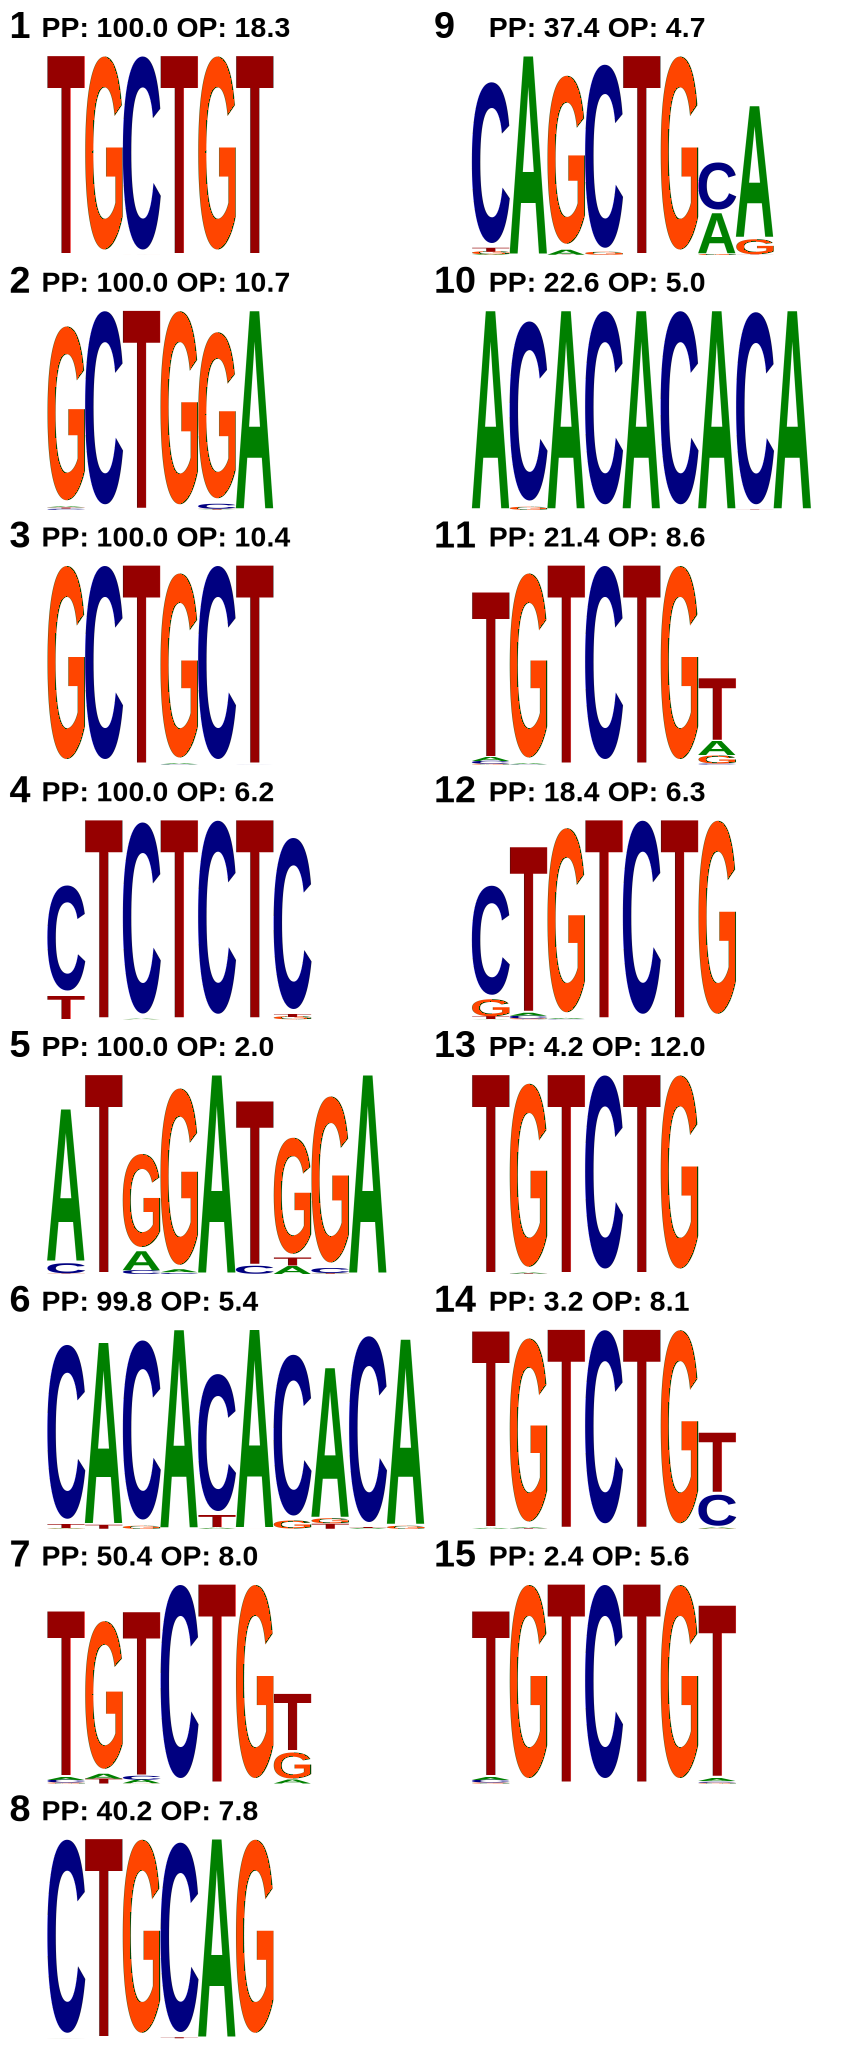
\includegraphics[width=.5\textwidth]{rys/sib_e_srcs.png}}    
    \caption{{\bf PWM sources detected in sibling differential nucleosome positions.}}
    PWMs presented as sequence logos with letter height proportional to position informational content\/emission probability.
    
    PP: Posterior prevalence; proportion of models within the compressed maximum a posteriori ensemble which have this PWM as a signal source

    OP: Observation prevalence; mean proportion of observed position sequences this sequence is used to explain, over all posterior samples

    Methods in \autoref{ssec:rysBMI}.
    Code in \autoref{ssec:dif_pos_learner}.
    \label{sibmotifs}
\end{figure}

\begin{figure}[!h]
    \makebox[\textwidth][c]{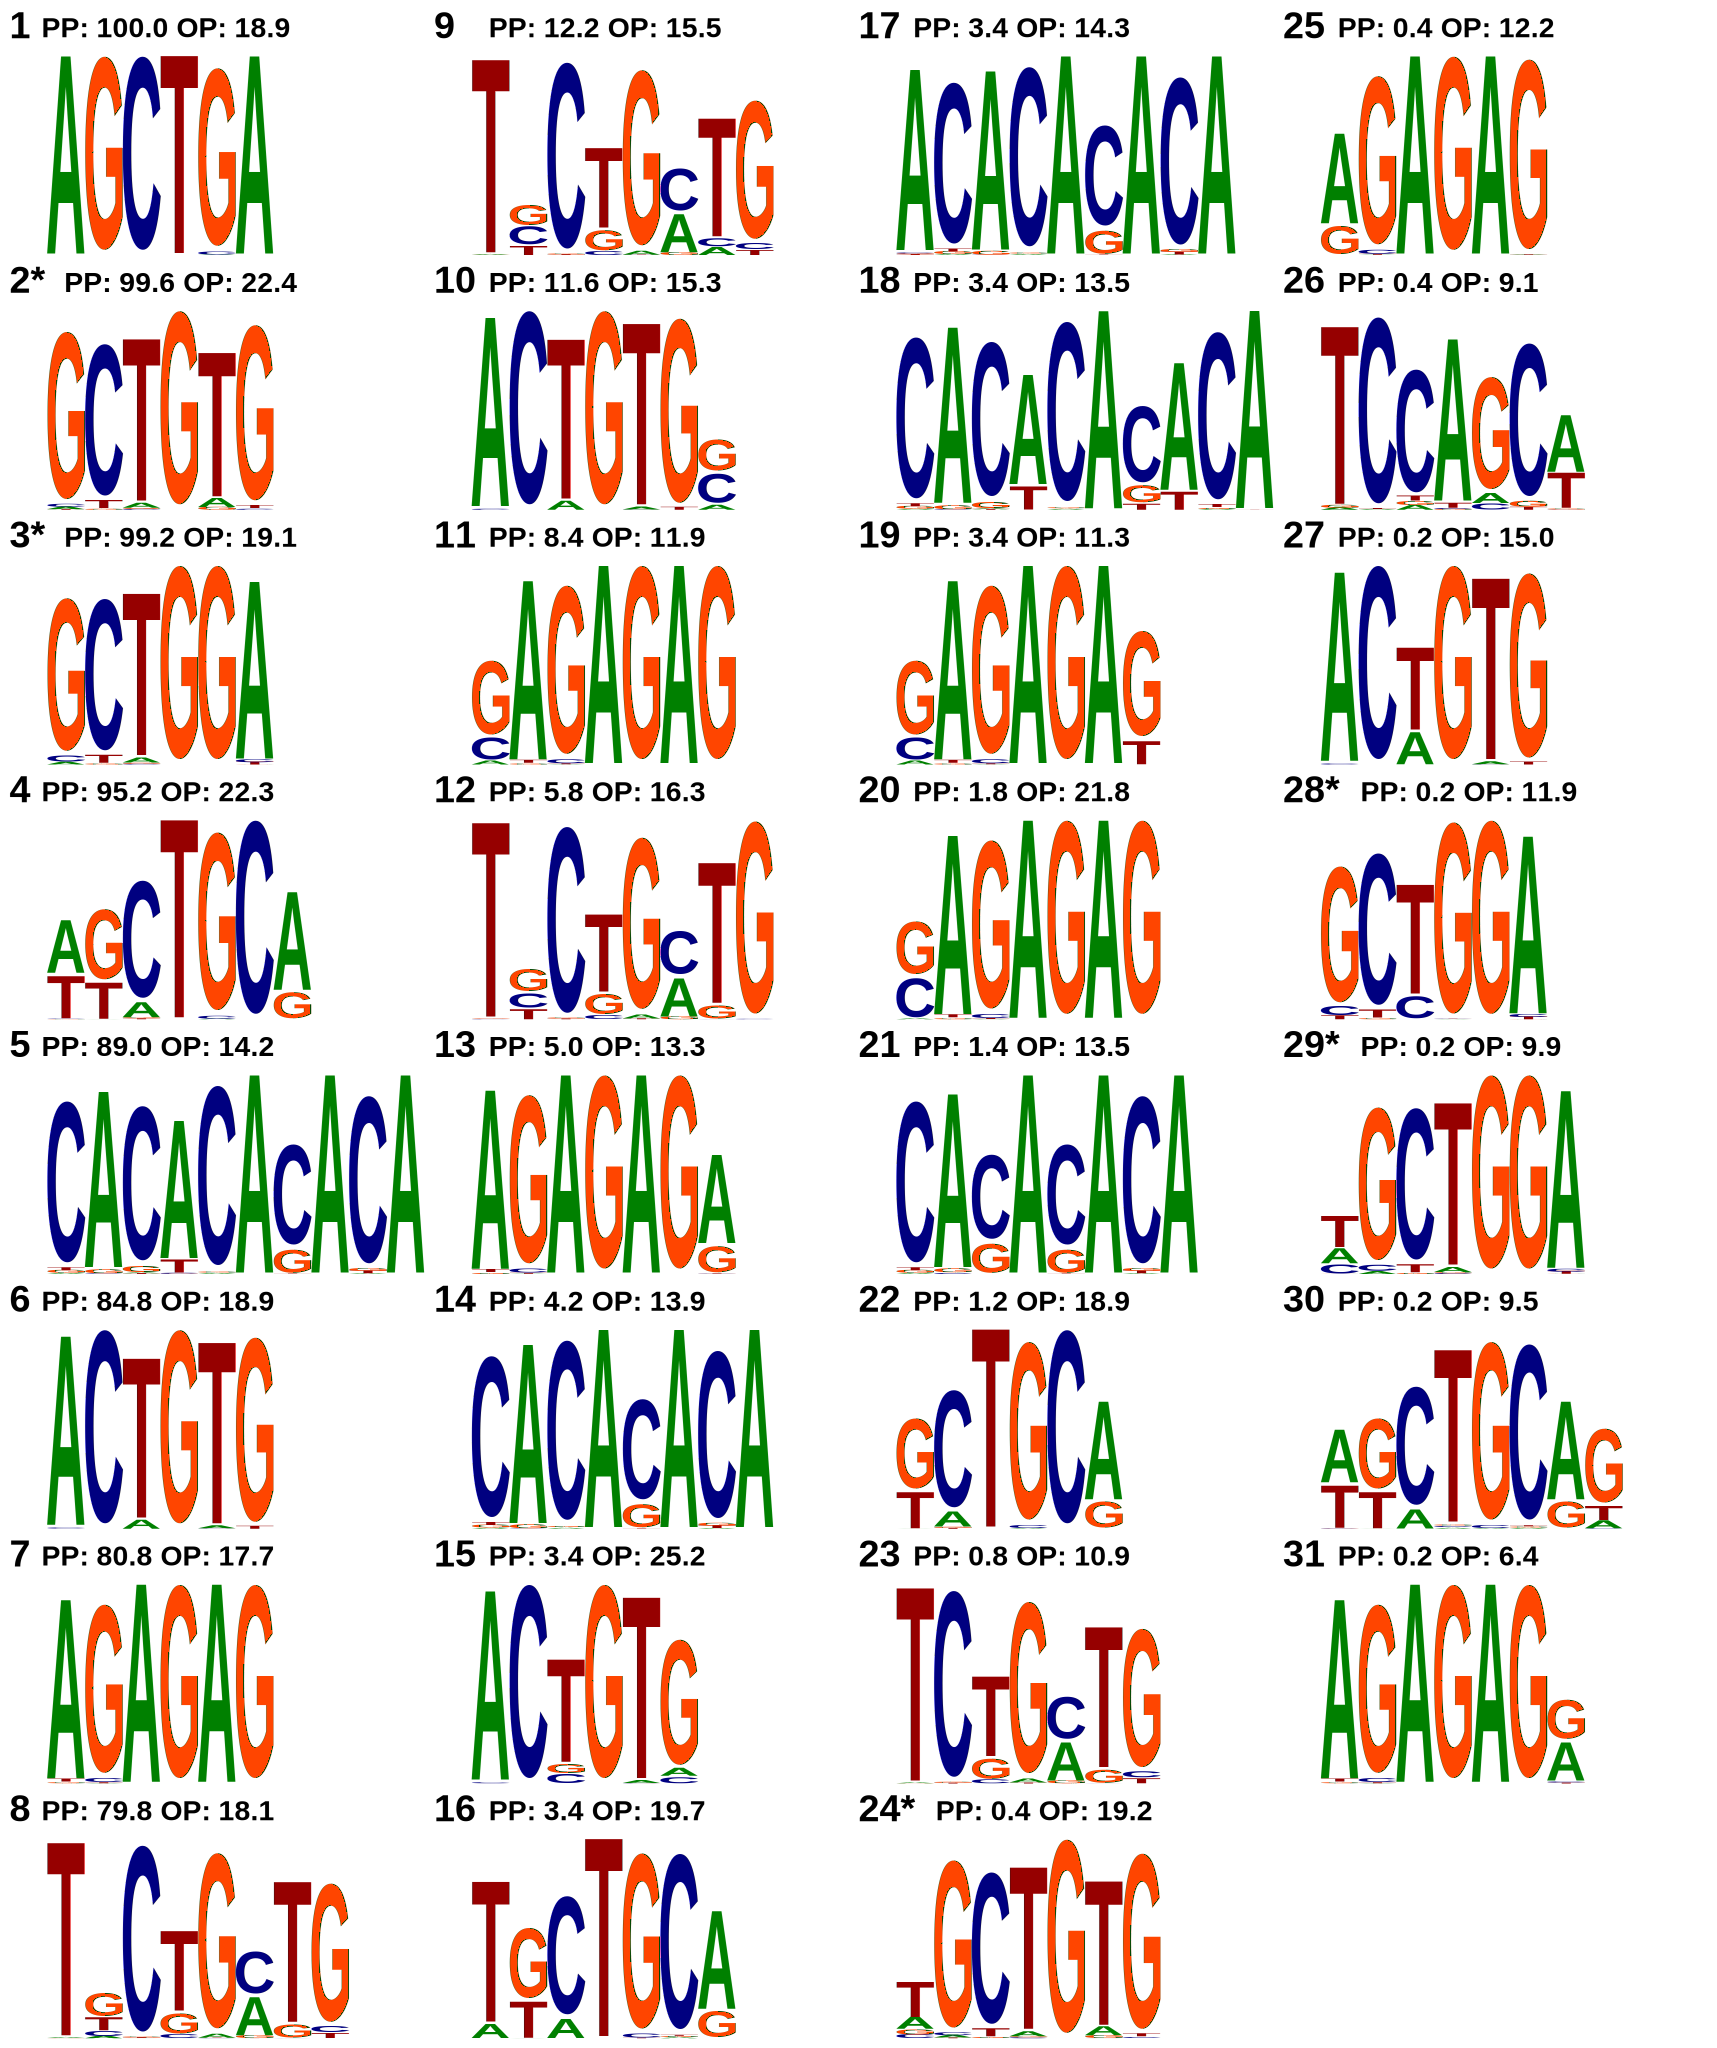
\includegraphics[width=1.\textwidth]{rys/rys_e_srcs.png}}    
    \caption{{\bf PWM sources detected in \textit{rys} mutant differential sources.}}
    PWMs presented as sequence logos with letter height proportional to position informational content\/emission probability.
    
    PP: Posterior prevalence; proportion of models within the compressed maximum a posteriori ensemble which have this PWM as a signal source

    OP: Observation prevalence; mean proportion of observed position sequences this sequence is used to explain, over all posterior samples
    
    Methods in \autoref{ssec:rysBMI}.
    Code in \autoref{ssec:dif_pos_learner}.
    \label{rysmotifs}
\end{figure}

\FloatBarrier

\section{Discussion}
We began our investigations by revising the original description of the \textit{rys} mutant CMZ phenotype. The apparently increased size of the CMZ in \textit{rys} mutants, relative to siblings, is produced as an effect of one or more of the following phenomena:

\begin{enumerate}
\item\label{inapret} Inappropriately retained RPCs in animals older than 7dpf
\item\label{specfail} Reduced neural population of the specified central retina, relative to the CMZ
\item\label{chromo} Expanded and spread-out RPC nuclei
\end{enumerate}

The first two effects are consistent with RPCs failing to specify as particular retinal neural lineages, demonstrated by retention of early progentior markers in these cells. \textit{rys} RPCs are not, however, arrested in cell cycle. Unlike systems where elevated polyadenylated histone transcript levels resulting in cell cyle arrest \cite{Kari2013}, we find that the mitotic activity of these cells actually accelerates under an overabundance of polyadenylated H2A and H2B transcript. We therefore suggest that the \textit{rys} phenotype is best characterised by chromatin disorganisation (phenomenon \ref{chromo}) and a failure of RPCs to correctly specify (which covers phenomena \ref{inapret} and \ref{specfail}) as retinal neural subtypes. The enlarged appearance of the CMZ is a result of these effects, and not a general increase in the CMZ population, RPC cytoplasmic volume\footnote{That is, alone, without an increase in nucleus size. We did not directly measure this parameter.}, or other variables. 

Moreover, in identifying npat as the lesioned gene underlying the \textit{rys} phenotype, we nominate a plausible macromolecular mechanism underlying phenomenon \ref{chromo} which could produce phenomena \ref{inapret} and \ref{specfail}. Mutant npat's effects on cell-cycle dependent histone transcription and stability may result in abberrant nucleosome positioning within proliferating cells, by altering the pool of histone proteins available for nucleosome formation. We posit that this is what causes the observed loss of a subpopulation of sibling nucleosome positions in \textit{rys}, together with the gain of novel, abberant positions. When we investigated whether the sequences of these subpopulations were better modelled by separate emissions processes than a shared emissions process, we found substantial evidence in favour of separate emissions processes, suggesting that nucleosome localisation to unique \textit{rys} positions occurs by different mechanisms than those unique to sibs. Interestingly, the PWM signals we detected in this differential nucleosome position set suggest some detail as to how changes in histone expression might result in the observed nuclear disorganisation of \textit{rys}. The observation that the background models explain the positions unique to siblings better than those unique to mutant \textit{rys} strongly suggests that sequence preference is less important in the process generating sibling positions than in the one generating mutant positions.

The relative importance of primary sequence in nucleosome positioning has been hotly debated; some have advocated for a nucleosome positioning code intrinsic to primary sequence \cite{Kaplan2009}, while others have disavowed the existence of any such code \cite{Zhang2009}. In general, the nucleosome dynamics community has moved on from these discussions in favour of emphasis on rotational sequence preferences \cite{Tolstorukov2007} and translational nucleosome positioning by \textit{trans}-acting factors \cite{Klages-Mundt2018}; a common interpretation of the earlier debate is that sequence preferences tend to dominate only at limiting concentrations of histones, when chromatin formation is rare \cite{Pointner2013}. The fact that sequence preference is less explanatory for the sibling positions than for the mutant ones is suggestive against this background. It seems likely that the shifted and novel nucleosome positions observed in mutants reflects all of the following:

\begin{enumerate}
    \item The appearance of nucleosomes with aberrant subunit composition
    \item A loss of translational control over \textit{rys} mutant nucleosomes by \textit{trans}-acting factors
    \item The limiting concentration of aberrantly-expressed nucleosomes, resulting in increased influence of ``default'' sequence-preference positioning
\end{enumerate}

All of the above could plausibly be caused by disrupted histone expression arising from altered npat activity. As regulation of chromatin dynamics is known to be important for both replication timing \cite{Gilbert2010} and cell identity and fate \cite{Serrano2013}, altered chromatin architecture could explain how mutated npat protein produces the observed shift in proliferative activity and failure of RPCs to specify, via altered histone expression. Moreover, chromatin density has recently been specifically implicated as fundamentally involved in the process by which pluripotent cells restrict gene expression to achieve their stable specified fates \cite{Golkaram2017}; it may be this overall process which has been disrupted in mutant \textit{rys}.

It is possible that the sequence-level inference is compromised by the ad-hoc nature of the sampler used in our nested sampling procedure. For reasons explained in \autoref{chap:BMI}, the ICA model structure makes euclidean space representations difficult, and ensuring sampling is in detailed balance may not be possible, given changing PWM signal lengths. We suggest that it is appropriate to magnify our error estimate by several of magnitude as a consequence. A conservative estimate of 100-fold more error than estimated, this has the effect of reducing the significance of the result from 527 to 5.27 standard deviations, which is still above the typical 5$\sigma$ significance typically accepted as a discovery in the physical sciences. We conclude that it is far more likely that the differential nucleosome populations found in \textit{rys} mutants and their phenotypically normal siblings are the result of separate generative processes. It is also possible that our identification of the differential subset of nucleosome positions with the disordered chromatin present in \textit{rys} RPCs is inaccurate. We have not conducted a full survey of \textit{rys} proliferative niches, and it is not clear how widely affected other cell types might be. Still, within the retina, only proliferative cells display the chromatin phenotype, and it is on this basis that we make the identification, which is the most parsimonious available. 

There are a number of important lacunae in this explanation. It remains unclear what form of the npat protein is expressed, if any. The overall effect on the expressed pool of histones in RPCs also remains uncharacterised. It is likely thhat there are macromolecules invovled in the \textit{rys} pathology which intermediate between the npat lesion and the observed chromatin phenotype which we have not examined. We suggest, however, that the overall effect on specification must be due to a failure of RPCs to organize chromatin for specification, and that, interestingly, this failure does not prevent proliferation. \textit{rys} therefore presents a useful model of the dissociability of proliferative and specificative behaviours in neural progenitors, which has recently been documented elsewhere in the developing \textit{D. rerio} retina \cite{Engerer2017}. Given the methodological limitations we encountered in probing protein expression in \textit{rys} RPCs, the most interesting and productive avenues of research to pursue in \textit{rys} pertain to this chromatin organisation phenotype.  Further experimentation is required to determine how particular changes in chromosome organisation (e.g. alterations in 3-dimensional chromatin organisation of gene expression, number of replication foci, etc.) produce specific features of the \textit{rys} phenotype. 

The zebrafish \textit{rys} mutant model provides a unique opportunity to study the role of a human NPAT homologue in a complete, developing tissue. This has previously proven difficult using mouse Npat, proviral inactivation of which resulted in early embryonic arrest, prior to tissue formation \cite{DiFruscio1997}. The survival and development of \textit{rys} mutant embryos beyond this stage may reflect the presence of wild-type npat transcript contributed maternally \cite{Harvey2013}; \textit{rys} mutants nevertheless do not survive beyond metapmorhosis (\textasciitilde{}21dpf), so npat seems to be similarly obligatory for normal development in zebrafish, if over a longer timeframe. Still, we observed many differences between the function of npat in zebrafish and documented effects in other vertebrates, which require some explication.

As teleost fish are known to have undergone whole-genome duplication subsequent to their radiation from vertebrates, it is possible that zebrafish may have multiple npat paralogues. We have excluded this possibility by failing to identify any significantly similar CDS sequences in the Zv9 zebrafish genome using BLAST, and the synteny analysis in \autoref{synteny}. The zebrafish npat gene does have a substantially different genomic context from human NPAT, however: it is not associated with the eponymous ATM locus (which has been duplicated, and is present in this duplicate form elsewhere on chromosome 15). ATM’s 5’ position is, in zebrafish, occupied by hif1al, with the intergenic region lacking canonical E2F promoter sites. Of the 80 vertebrate genomes currently available from Ensembl, this organisation is shared only with the cave fish (A. mexicanus), with the human-like ATM-NPAT association preserved in all other species. This apparently evolutionarily novel genomic organisation for npat may be responsible for some of the differences in npat function we report here, relative to its homologues.

We identified alterations in histone mRNA transcription and 3’ end processing as likely mechanistically involved in the \textit{rys} phenotype. In both 6 and 8 dpf \textit{rys} larvae as well as npat-morpholino treated 1dpf embryos, we observe increased abundances of total and polyadenylated histone transcripts. The mechanism by which these effects are produced in \textit{rys} remains unclear. The increases in histone transcript abundance observed in both mutant and morpholino-treated animals are at odds with observations that NPAT knockouts display decreases in histone transcription \cite{Ye2003}, and that the destruction of CDK phosphorylation sites on NPAT protein, which would be the case in the putatively truncated \textit{rys} npat protein, result in similar declines in histone transcript abundance \cite{Ma2000,Mitra2009}. This implies the role of zebrafish npat in regulating histone transcription differs from human NPAT. We are unable to determine from these data whether the overall increases in histone transcript abundance are a consequence of increased histone transcription, or of the greater stability of improperly polyadenylated histone transcript. The increased abundance of polyadenylated transcript in \textit{rys} mutants and npat morpholino-treated embryos is consistent with the observed role of NPAT in recruiting CDK9 to replication-dependent histone gene clusters, known to be important in generating the normal stem-loop structure at the 3’ end of these transcripts \cite{Pirngruber2009}, suggesting that this role is conserved in zebrafish. It is also possible that particular histone genes give rise to polyadenylated transcripts in zebrafish, as observed in a variety of cell lines \cite{Kari2013}. Increased transcription of these particular genes might also account for the observed increase in polyadenylated histone transcript abundance. Although increased abundance of polyadenylated histone transcript has been associated with both cell cycle arrest and differentiation \cite{Kari2013}, we found that in the \textit{rys} mutant CMZ, this was associated with altered cell cycle parameters, failure to differentiate, and ultimately, cell death by apoptosis. This suggests that the presence of polyadenylated histone transcripts are not directly related to particular cell cycle states or differentiated fates, but rather that a particular regime of coordination and control of the expression of polyadenylated and replication-dependent, stem-looped histone transcripts is required to achieve appropriate transitions between these states. In the case of \textit{rys}, this seems to be related to the effect of altered histone expression on chromatin structure.